\documentclass{article}
\usepackage{graphicx}
\graphicspath{ {./images/} }
 
\begin{document}


\section{Figure}

\begin{figure}[h]
\caption{Example \tt{jpg} image)}
\centering
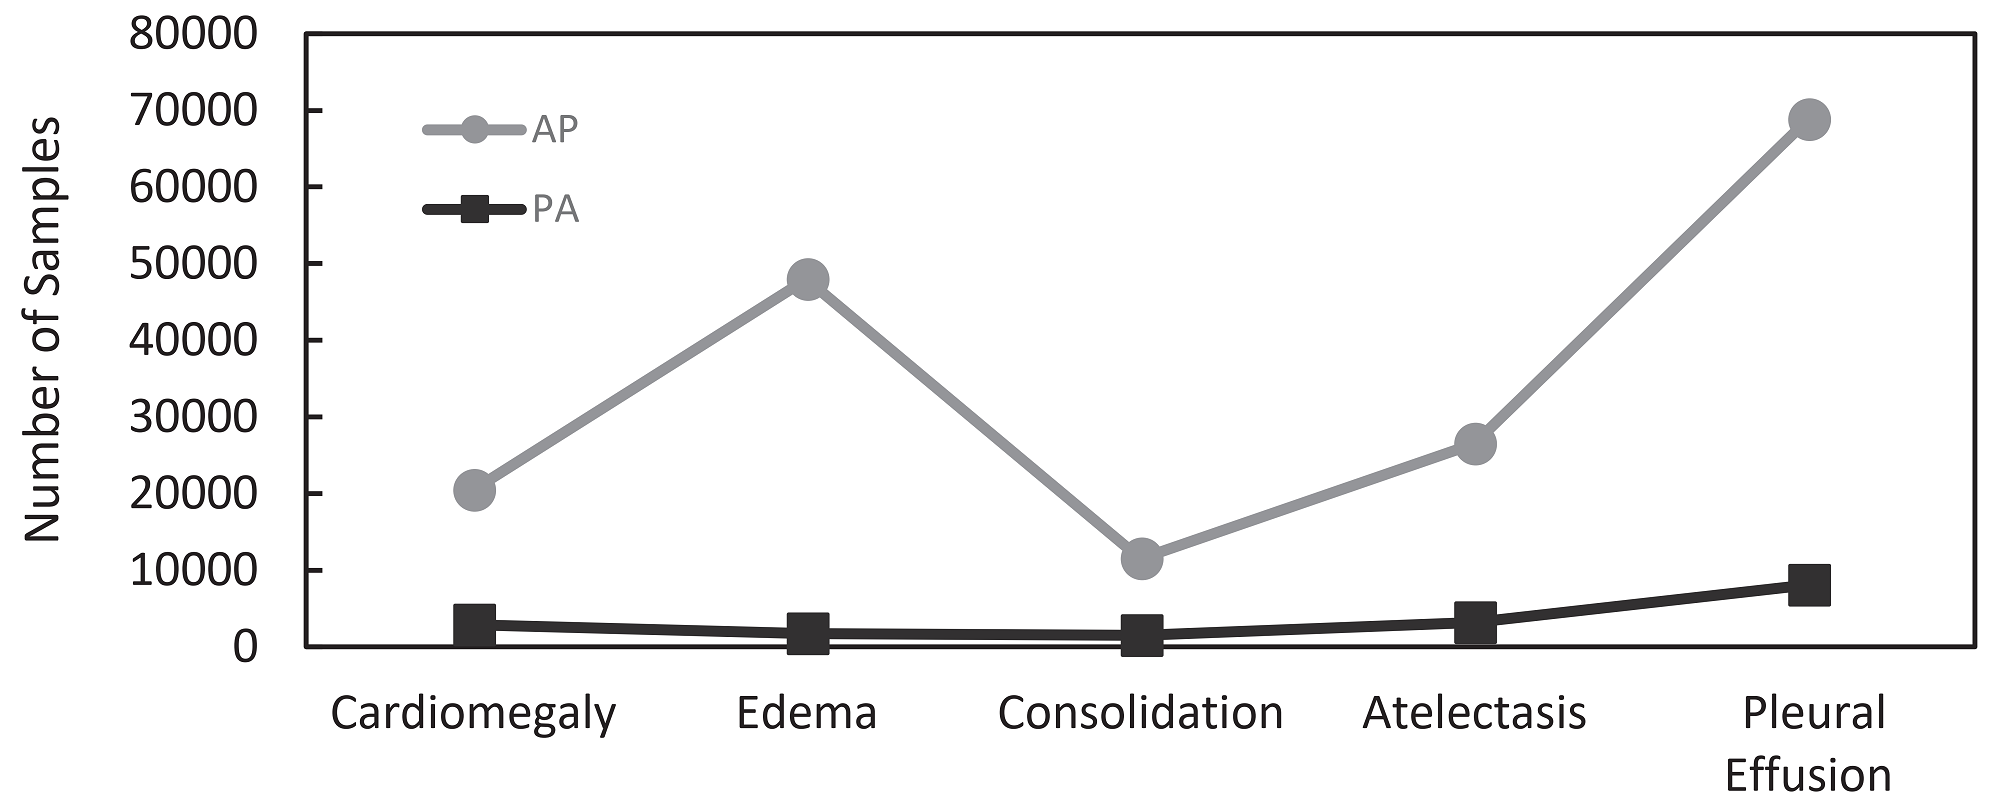
\includegraphics[width=0.9\textwidth]{observation_ap_pa_distribution.png}
\end{figure}
 
\begin{figure}[h]
\caption{Example \tt{pdf$\backslash$Vector} image)}
\centering
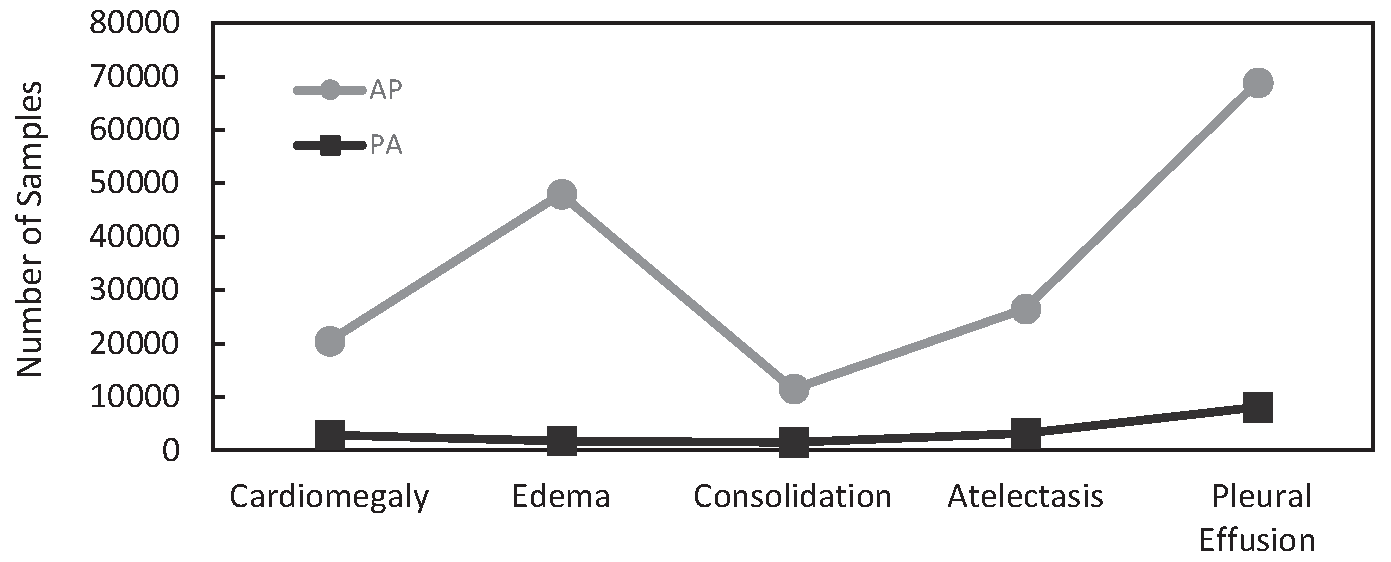
\includegraphics[width=0.9\textwidth]{observation_ap_pa_distribution.pdf}
\end{figure}

\section{Table}


\begin{table}[h]
\centering
\begin{tabular}{ |c c| }
\hline
 cell1 & cell2 \\ 
 cell4 & cell5 \\  
 cell7 & cell8 \\
\hline
\end{tabular}
\end{table}


\end{document}